% (c) Jakub Stejskal
% Master Thesis
% Performance Testing and Analysis of Qpid-Dispatch Router
% Chapter 4

\chapter{Analysis and Design}
\label{Analysis and Design}
MPT is generally designed for performance testing of Broker. However, with the service growth, the need for performance testing of Qpid-Dispatch comes. This Chapter is focused on two things: firstly, analyze Qpid-Dispatch service, describe its capabilities and methodology. Secondly describe design of Topology Generator and Qpid-Dispatch Performance Module for MPT.

\section{Qpid-Dispatch Router}
Qpid-Dispatch is a lightweight AMQP message router for building scalable available and performant messaging networks. With respect to ISO/OSI\footnotemark{} model, this router is an application layer program running as a normal user program or as a daemon. Key features of Qpid-Dispatch are:

\begin{itemize}
	\setlength\itemsep{0em}
	\item Connects clients and brokers into an internet-scale messaging network with uniform addressing.
	\item Supports high-performance direct messaging.
	\item Uses redundant network paths to route around failures.
	\item Streamlines the management of large deployments.
\end{itemize}
The following theory about Qpid-Dispatch router is based on knowledge available~in~\cite{RH:Interconnect}.

\footnotetext{ISO/OSI - \url{http://www.studytonight.com/computer-networks/complete-osi-model}}

\subsection{Theory of Operation}
The router accepts AMQP connections from senders and receivers and create AMQP connections to Message Brokers or similar AMQP-based services. Through this connection is sender able to reach message receiver, which can be another client in the network or message broker. The client can exchange messages directly with another client without involving a broker at all. The router classifies incoming messages and routers them between senders and receivers. The router is designed to be deployed in topologies of multiple routers, preferably with redundant paths to provide continued connectivity in the case of any router in the network fails. For routing Qpid-Dispatch uses link-state routing protocols\footnotemark{} and algorithms similar to OSPF or IS-IS to calculate best path (path with the lowest cost) from sender to receiver through the whole network and to recover from failures.

\footnotetext{Link-state protocols - \url{https://www.certificationkits.com/cisco-certification/ccna-articles/cisco-ccna-intro-to-routing-basics/cisco-ccna-link-state-routing-protocols/}}

\subsection{Addresses and Connections}
\label{Addresses and Connections}
Qpid-Dispatch is able to connects clients servers, AMQP services, and other router implementations through network connections. The router provides multiple components and settings for specifying service on the other side of connection link.

\begin{description}
	\setlength\itemsep{0em}
	\item \textbf{Addresses\footnotemark{}}\,---\,are used to control the flow of messages across a network of routers. Addresses can specify messages and they are also used during the creation of links since links are bounded to specific address field of a source and a target. The addresses can refer to topics or queues that match multiple consumers to multiple producers. There are two types of addresses:
	\begin{itemize}
		\setlength\itemsep{0em}
		\item \textbf{mobile}\,---\,The address is a rendezvous between senders and receivers. The router is message distributor.
		\item \textbf{link route}	\,---\,The addresses defines a private messaging path between sender and receiver. The router only passes messages between end points.
	\end{itemize}
	\item \textbf{Listener}\,---\,accept client connections. Listeners has several types that are defined by their role:
	\begin{itemize}
		\setlength\itemsep{0em}
		\item \textbf{normal}\,---\,The connection is used for AMQP clients using normal message delivery.
		\item \textbf{inter-router}	\,---\,The connection is created to another router. Inter-router connection can only be establish over inter-route listeners.
		\item \textbf{route-container}	\,---\,The connection is established to a broker or other resource that holds known addresses.
	\end{itemize}
	\item \textbf{Connector}\,---\,used as an interface for create connection with brokers or other AMQP entities using connectors. Such as listeners, connector has several types that are defined by their role:
	\begin{itemize}
		\setlength\itemsep{0em}
		\item \textbf{normal}\,---\,The connection is used for AMQP clients using normal message delivery. The router will initiate the connection but links are created by the peer that accepts the connection.
		\item \emph{Inter-router} and \emph{route-container} modes are the same such as listener's modes.
	\end{itemize}
\end{description}

\footnotetext{Addresses in this discussion refer to AMQP protocol addresses, not to TCP/IP addresses.}

To ensure security the router uses \emph{SSL/TLS - Sockets Layer and Transport Layer Security}\footnote{SSL - \url{https://tools.ietf.org/html/rfc6101}; TLS - \url{https://tools.ietf.org/html/rfc5246}} protocol and related certificates and \emph{SASL - Simple Authentication and Security Layer}\footnotemark{} protocol mechanisms to encrypt and authenticate remote peers. Router listeners act as network servers and connectors act as network clients. Both connection components may be configured securely with SSL/TLS and SASL.

\footnotetext{SASL - \url{https://tools.ietf.org/html/rfc4422}}


\subsection{Message Routing}
\label{Message Routing}
Addresses have semantics associated with them. This semantics control how routers behave when they see the address being used. There are two ways how the router can routing messages based on addresses:

\begin{description}
	\setlength\itemsep{0em}
	\item \textbf{Routing pattern}\,---\,define the paths which message with a mobile address can take. Routing patterns can be used in both case of message delivery; with broker or directly through the router.
	\begin{itemize}
		\setlength\itemsep{0em}
		\item \textbf{Balanced}\,---\,An anycast\footnotemark{} method which allows multiple receivers to use the same address.
		\item \textbf{Closest}\,---\,An anycast method in which every message is sent along the shortest path to reach the destination.
		\item \textbf{Multicast}\,---\,method for send copy of the message to every receiver with the same address.
	\end{itemize}
	\item \textbf{Routing mechanism}\,---\,define the path to endpoint for message from sender to receiver.
	\begin{itemize}
		\setlength\itemsep{0em}
		\item \textbf{Message routed}\,---\,message delivery is done based on address in message's \emph{to} field. The router check destination address of the message and find the same address in its routing table. The message is sent to all links with that address.
		\item \textbf{Link routed}\,---\,this method uses same routing table like Message routing but the difference is that the routing occurs during the link-attach operation and link attaches are propagated along the appropriate path to the destination. It results into a chain of links from source to destination.
	\end{itemize}
\end{description}
Message may be delivered with various degrees of reliability such as \emph{at most once}, \emph{at least once} and \emph{exactly once}.

\footnotetext{Anycast vs. Multicast - Anycast method send data to every node in network. Multicast method send data only to specified group of nodes.}

\section{Automatic Topology Generator}
For various kind of messaging systems testing we needs multiple topologies with different components and setting. Creating and deploying the scenarios manually for each test scenario is slow and annoying, after few scenarios. Solution to this problem is divided into two parts: simple topology generator, that transform metadata, defined by user, into configuration files for each component contained in metadata, and automatic \emph{Ansible} scripts, which deploy whole topology to physical machines. User has to define metadata file, single file for whole topology instead of single file for each component, and then start Ansible script which ensure configuration files generation and deployment.


\subsection{Topology Components}
Messaging system consists of multiple components with specific role. In our case, testing topologies will consider clients, brokers, and routers. Clients refer to message senders and receivers and there is no need for specific configuration of each clients at all. Message settings is another case, but MPT deal with it as was mentioned at Chapter \ref{Messaging Performance Tool}.

\subsubsection*{Broker}
Broker configuration file offers various setting and protocols such as specialized queueing behaviors, message persistence, and manageability. The following list shows several capabilities of broker:

\begin{itemize}
	\setlength\itemsep{0em}
	\item \textbf{User access}\,---\,allows guest access or authentication access for users.
	\item \textbf{Multiple Protocol Support}\,---\,broker supports AMQP, MQTT, STOMP, OpenWire and Core protocols.
	\item \textbf{Connections}\,---\,can establish connection to another AMQP-based service such as another broker or router.
	\item \textbf{Queues}\,---\,user can specify new queues in configuration file or allow auto-create option.
	\item \textbf{Messaging types}\,---\,refer to approach how to deliver messages, examples are point-to-point and publish-subscribe approach.
	\item \textbf{Logging level}\,---\,broker offers to setup different logging levels.
\end{itemize}
However, broker configuration is not implemented yet, but design of automatic configuration generation will be shared with router configuration generation.

\subsubsection*{Router}
Just like broker configuration, router offer various types of configurations. The basics were explained in Subsections \ref{Addresses and Connections} and \ref{Message Routing}, but for better understanding of all capabilities I~recommend Qpid-Dispatch documentation \cite{RH:Interconnect}.

\subsection{Format of Input and Output}
Input structure should be user-friendly and easy to update even in case of large topologies. As input is choose one file called \texttt{config.yml} in \emph{YAML}\footnotemark{}  language, which is similar to JSON but it's better readable for humans. Generator needs information about all hosts in topology and which type of topology it should generate. For that purpose there is two attributes in configuration file; first is \emph{inventory path} which refer to location of \emph{Inventory}. Inventory is file, containing all hosts in topology in specific format. This format is available in Appendix \ref{AP:Inventory}. It is simple configuration file with enumeration of host names and their IP addresses. Second attribute is which type of topology it should generate. There user can specify one of the simple types of graph, such as line, circle, complete, etc., which do not need any other information except Inventory or he can specify path to graph metadata. Graph metadata are more described in Subsection \ref{Graph Metadata}.

On the other hand, output format should be easy for automatic parsing. The best format for machine parsing is JSON or YAML format, since both of them are loaded with same functions in ansible. Output of the generator will be passed to ansible script immediately after creation without any user intervention. However, user should have option to see generator output in YAML format, because in case of larger topologies JSON is badly readable for human eyes. Output will be one JSON file with variables for template. Each node from Inventory will have its own variables separated from variables of other nodes. Scheme of the input and output for Topology Generator you can see in the Figure \ref{fig:generator}.

\begin{figure}[H]
  \centering
  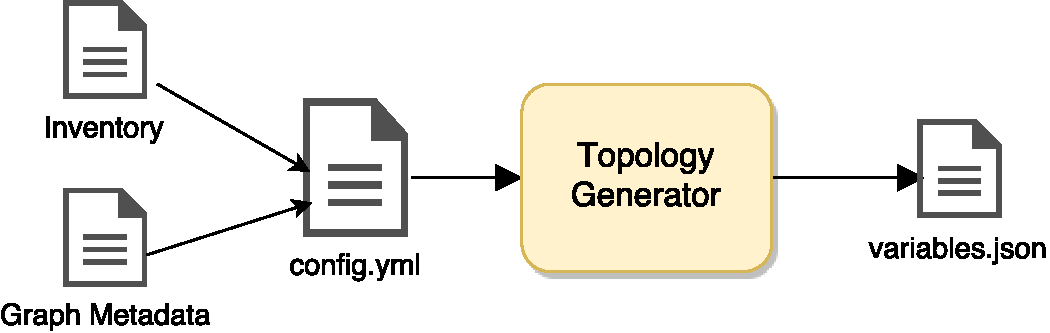
\includegraphics[width=10cm]{obrazky-figures/generator.pdf}
  \caption{Topology Generator with input and output scheme.}
  \label{fig:generator}
\end{figure}

\footnotetext{YAML - \url{http://docs.ansible.com/ansible/latest/YAMLSyntax.html}}

\subsection{Graph Metadata}
\label{Graph Metadata}
At first, we should specify technology which will be used for implementation of Topology Generator. \emph{NetworkX} is a Python package for creation and manipulation of complex networks. This package offer features for creating graphs, multigraphs, random graph generators, plot created graph, and etc. NetworkX also offers graph import and export in YAML structured file. This type of file is very useful as graph metadata, simple example of this file is shown in Appendix \ref{AP:Graph Metadata}.

Here user can specify any setting for each node. For example, user can specify listener for router\,1, and connector for router\,2 as you can see on the example below.

\begin{verbatim}
---
directed: false
graph: {}
nodes:
- type: router
  id: router1
  listener:
  	- host: 0.0.0.0
  	  port: 1080
  	  role: inter-router
- type: router
  id: router2
  connector:
  	- name: router1
  	  host: router1
  	  port: 5675
  	  role: inter-router
multigraph: false
\end{verbatim}
From this metadata NetworkX create two nodes with type, id, and listener or connector attributes. This attributes will be used for generating configuration files for each node. All possible attributes that user can specify for each node is available in Appendix \ref{AP:Qpid-Dispatch Configuration File Template}.

However, specifying all attributes of each node is not very user-friendly approach, especially in case of large topologies. User could only specify nodes, and links between them and generator will add all necessary attributes for establish connection between nodes. Example of this metadata file you can see in Appendix \ref{AP:Graph Metadata}.

\subsection{Topology Deployment}
Every node specified in Inventory has to receive proper configuration files for services running on it. This job will be handled by Ansible, since it can connect to all nodes from Inventory and copy configuration files to proper destination folders. Ansible script load data from Topology Generator and create configuration files based on loaded variables and common template for Qpid-Dispatch. Created file will be sent to proper node based on node name from Inventory, which has to be same like router name specified in generated variables. You can see scheme of configuration deployment in the Figure \ref{fig:deployment}.

\begin{figure}[H]
  \centering
  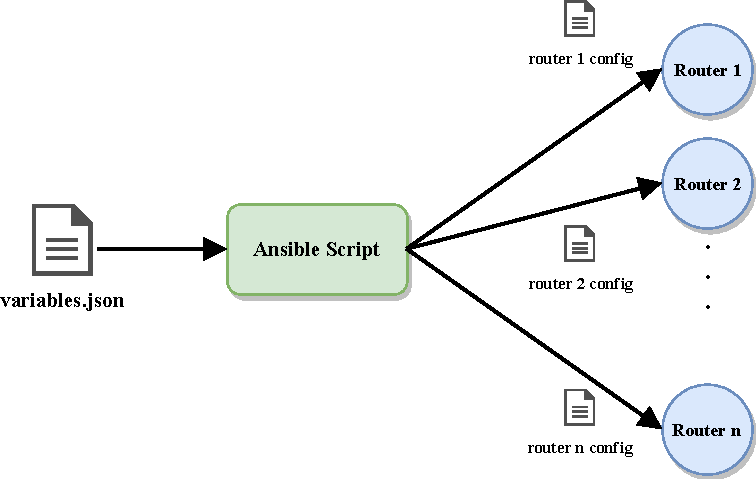
\includegraphics[width=12cm]{obrazky-figures/deployment.pdf}
  \caption{Scheme of configuration files deployment to the nodes.}
  \label{fig:deployment}
\end{figure}


\section{Qpid-Dispatch Performance Module}
We saw architecture of Maesto in the Figure \ref{fig:msg_perf_tool}. This architecture cannot use all performance testing and network recovery possibilities of router. For better performance analysis and measurements is necessary to design and implement additional functionality for MPT.

\begin{figure}[H]
	\centering
	\begin{minipage}{6.5 cm}
\subfloat[Network with router agent.\label{fig:agent_1}]{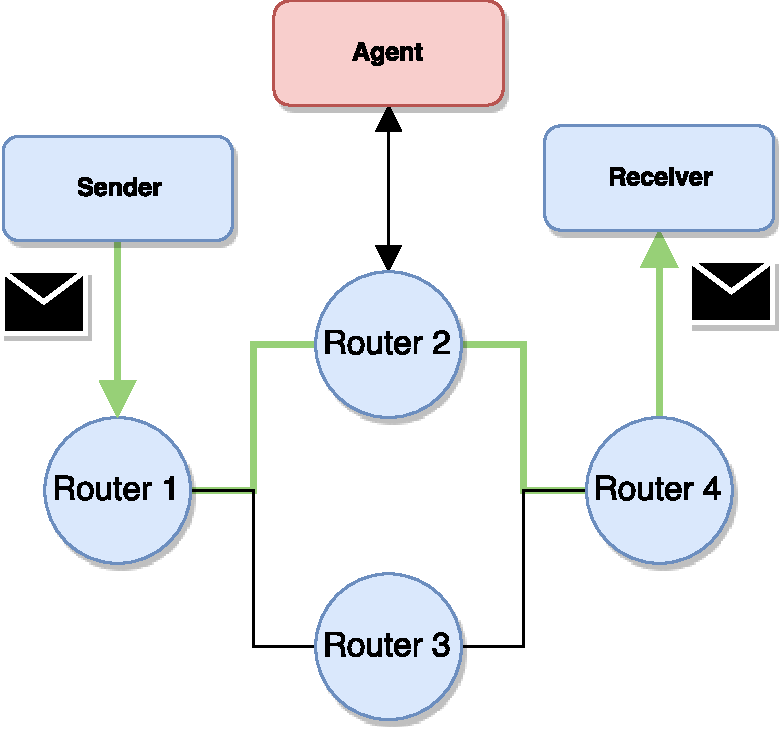
\includegraphics[width=1\linewidth]{obrazky-figures/agent_1.pdf}}
\end{minipage}
	\begin{minipage}{6.5 cm}
\subfloat[Router shut-down demonstration.\label{fig:agent_2}]{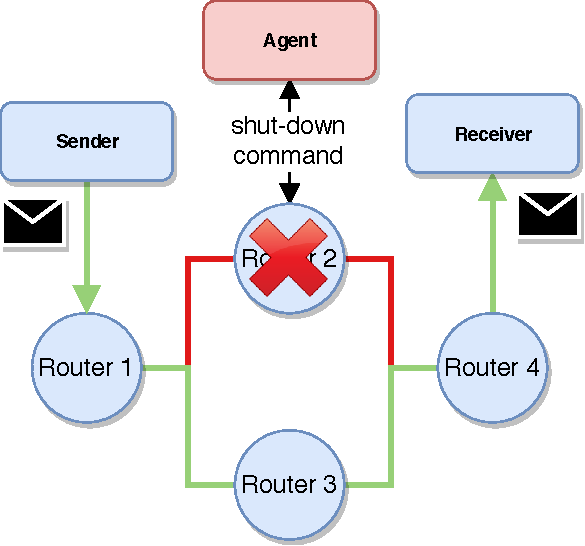
\includegraphics[width=1\linewidth]{obrazky-figures/agent_2.pdf}}
\end{minipage}

	\caption[Simple network with active router agent.]{Simple network with router shut-down demonstration.}\label{fig:agent}
\end{figure}

In the Figure \ref{fig:msg_perf_tool_update} is updated version of Maestro architecture. Proper performance testing of router and network analysis with few routers needs some kind of agent, which can manipulate each node. In particular, MPT should be able to shut down one of the router node and Collected Data Format about network behavior during this situation. This actions will be handled by new back-end component called \emph{Agent}.

\begin{figure}[H]
  \centering
  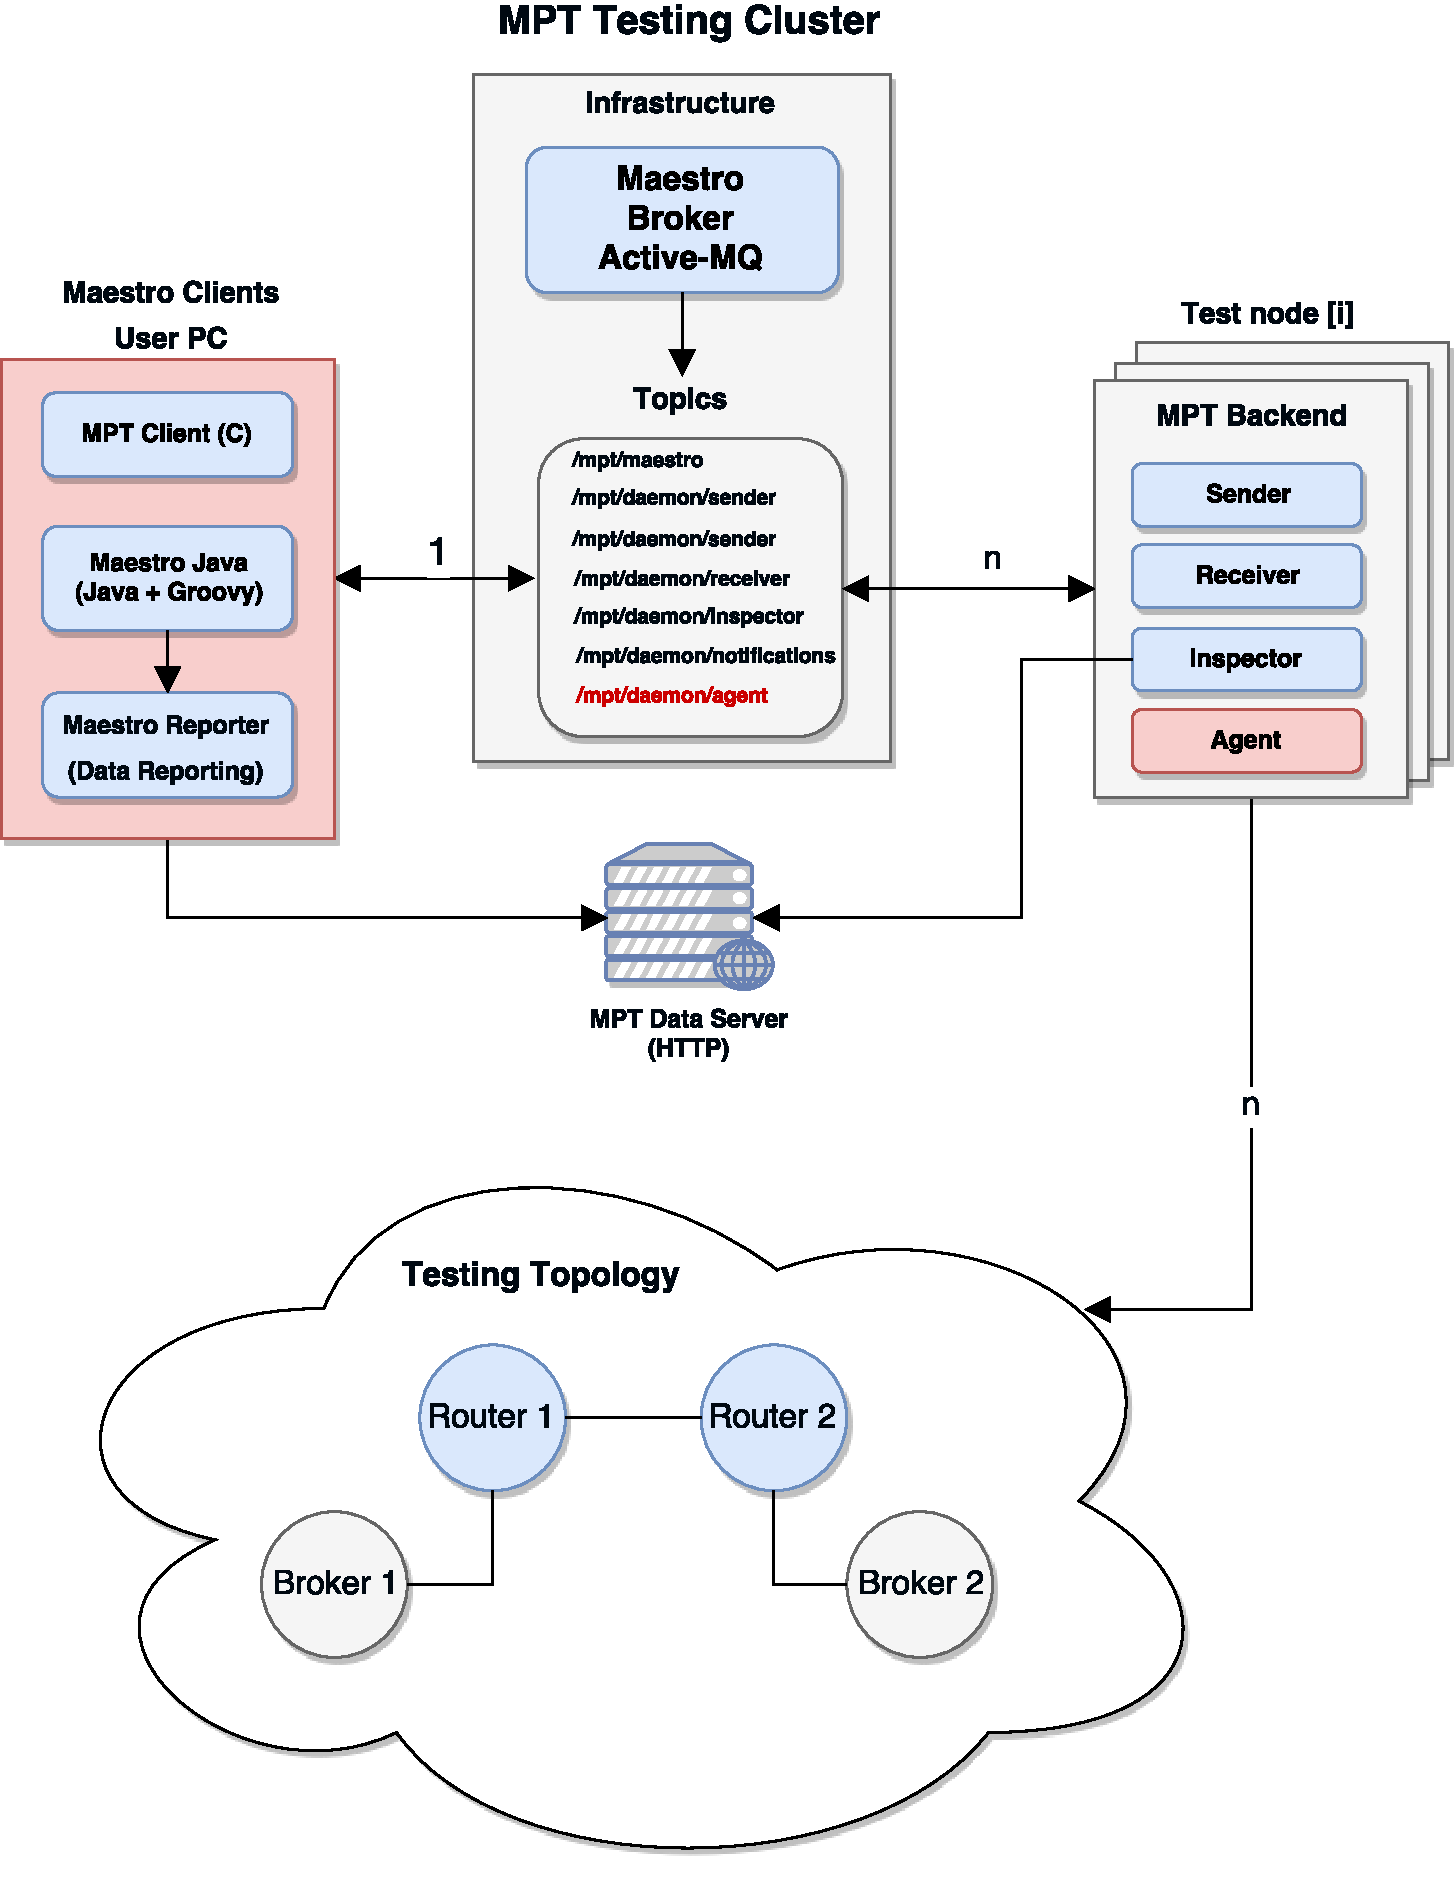
\includegraphics[width=15cm]{obrazky-figures/msg_perf_tool_for_router.pdf}
  \caption{Architecture of updated Maestro for testing of Qpid-dispatch router.}
  \label{fig:msg_perf_tool_update}
\end{figure}

In the Figure \ref{fig:agent_1} you can see simple scheme of topology and one agent monitoring router\,2. Communication passing through router\,2 and message is delivered to receiver without problems. Shut-down demonstration is in the Figure \ref{fig:agent_2} where you can see command from agent to router\,2. In that case, the network will choose redundant link through router\,3. This scenario can answer the question \emph{How this incident influence latency between sender and receiver?}

Another part is communication inside Maestro cluster with new component. Communication between cluster back-end and user client is happening through Maestro Broker and for proper message distribution new topic has to be added. As was mentioned in Section \ref{Collected Data Format}, Maestro Clients communicating with back-end via specialized command. Router Agent will accept new set of commands for router control. This set has to be added to existing Maestro Clients. All additional components or components for update are highlighted by red color in the Figure \ref{fig:msg_perf_tool_update}. Example of simple testing topology consists of two routers and two brokers is also available in that Figure.



\subsection{Communication with Agent}
\label{Communication with Agent}
For communication inside Maestro testing cluster is used The Maestro Protocol which was described in Subsection \ref{Communication Between Components}. MPT Clients has to know how to communicate with new component in the cluster and for this its necessary to add new communication commands. The following list shows new commands which should be added:

\begin{itemize}
	\setlength\itemsep{0em}
	\item \textbf{MAESTRO\_NOTE\_START\_ROUTER (17)}\,---\,start specific router in the network.
	\item \textbf{MAESTRO\_NOTE\_STOP\_ROUTER (18)}\,---\,stop specific router in the network.
	\item \textbf{MAESTRO\_NOTE\_RESTART\_ROUTER (19)}\,---\,restart specific router in the network.
	\item \textbf{MAESTRO\_NOTE\_ROUTE\_ERROR (20)}\,---\,signals error during routing.
\end{itemize}

\subsection{Collected Data}
\label{Collected Data}
Collected data Format for new module will be almost same as it is in current version of MPT (described in Subsection \ref{Collected Data Format}). Since Qpid-Dispatch is written in C, there is no need to monitoring Java memory space. The following list shows updated data collected by Inspector:

\begin{itemize}
	\setlength\itemsep{0em}
	\item \textbf{Timestamp}\,---\,the date and time for the data sample in the format YYYY-MM-DD hh:mm:ss using the W3C defined standard for datetime.
	\item \textbf{Load}\,---\,size of system load.
	\item \textbf{Open file descriptors}\,---\,number of opened filed descriptors.
	\item \textbf{Free file descriptors}\,---\,number of free file descriptors.
	\item \textbf{Free memory}\,---\,free physical memory.
	\item \textbf{Free swap memory}\,---\,swap free memory.
	\item \textbf{Swap committed}\,---\,swap committed memory.
	\item \textbf{Consumers}\,---\,number of active connectors connected to the router.
	\item \textbf{Message amount}\,---\,amount of routered messages.
\end{itemize}
Data collected by senders and receivers remains same as its in current version of MPT.
